Optimization is such an important tool that it deserves a set of notes in itself. All problems in model training essentially stems from non-ideal optimization. Knowing the strengths and weaknesses of each optimizer allows you to diagnose which ones to use. 

Generally, we (non-exclusively) categorize optimization algorithms as such: 
\begin{enumerate}
  \item \textit{Convex}? Convex optimization is pretty easy to solve and has been studied extensively. 
  \item \textit{Constrained}? Is the parameter space constrained to a certain manifold? 
  \item \textit{Order}. Do we use derivatives at all? First-order derivatives (gradient)? Second-order (Hessian)? 
\end{enumerate}

These algorithms try to solve the following potential problems. 
\begin{enumerate}
  \item \textit{Convergence}. Do we converge to some point? 
  \item \textit{Optimality}. Is this point close to the true global minima?  
  \item \textit{Efficiency}. Can we iterate efficiently? 
\end{enumerate} 

As a benchmark test, the following function will be used a lot. 

\begin{definition}[Rosenbrock Function]
  The \textbf{Rosenbrock function} is defined 
  \begin{equation}
    f(x, y) = (a - x)^2 + b (y - x^2)^2
  \end{equation}
  which has a global minimum at $(a, b)$. 

  \begin{figure}[H]
    \centering 
    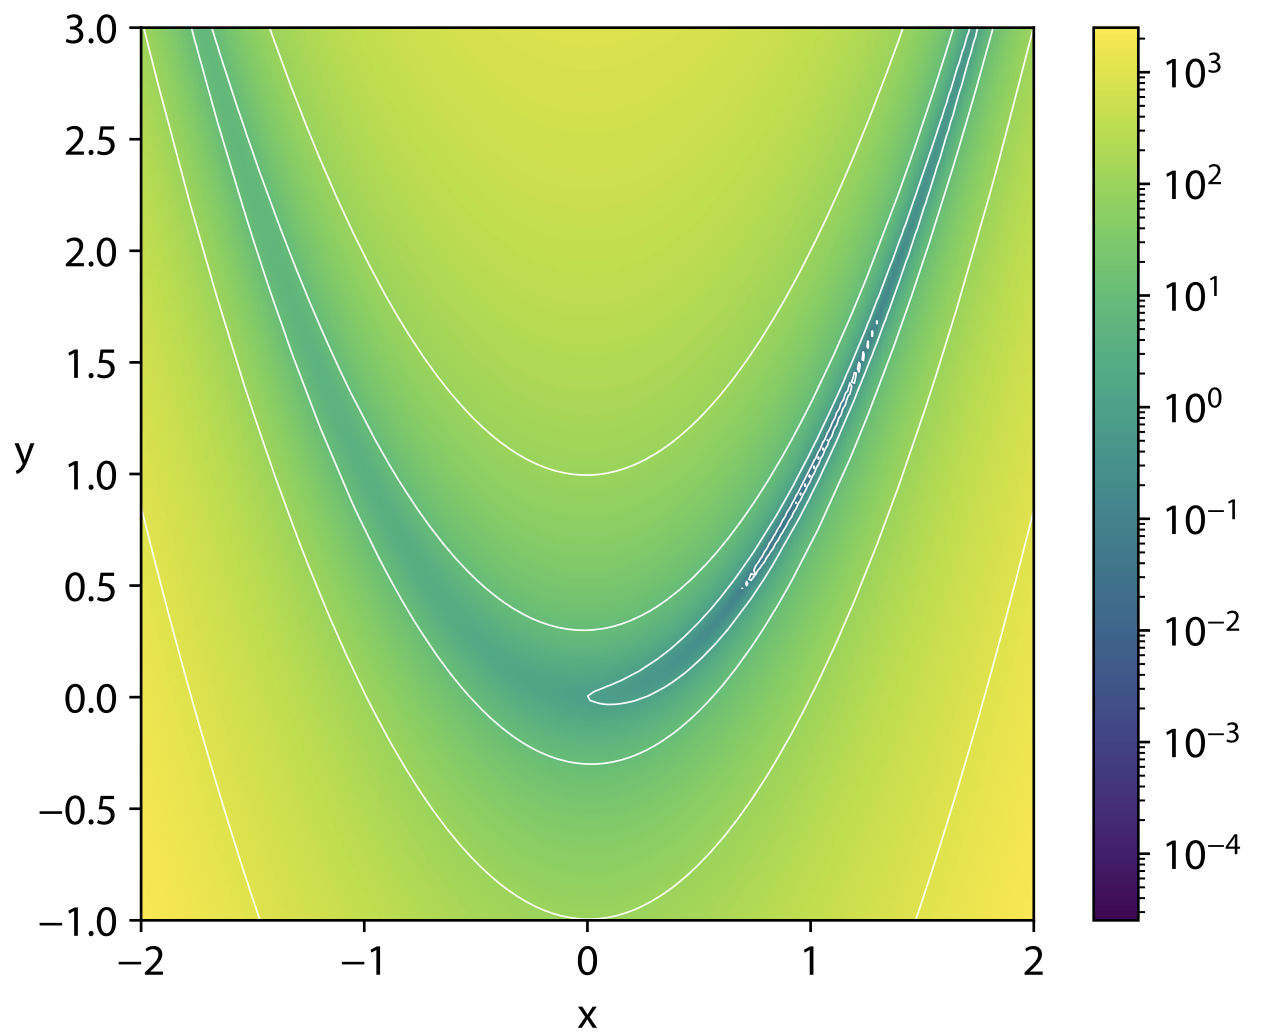
\includegraphics[scale=0.4]{img/rosenbrock.png}
    \caption{Typically, we set $a = 1, b = 100$. } 
    \label{fig:rosenbrock}
  \end{figure}
\end{definition}

